\documentclass{standalone}
\usepackage{tikz}

\begin{document}
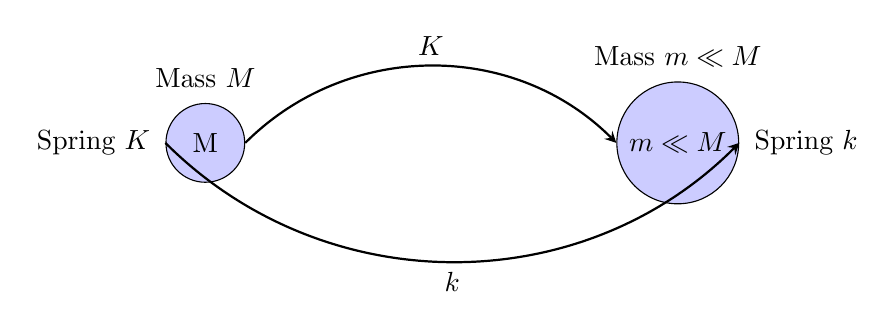
\begin{tikzpicture}[scale=1.5]
    % Define styles for nodes and edges
    \tikzset{
        mass/.style={circle, draw, fill=blue!20, minimum size=1cm},
        spring/.style={thick, ->, >=stealth}
    }

    % Position the masses
    \node[mass] (M) at (0,0) {M};
    \node[mass] (m) at (4,0) {$m \ll M$};

    % Draw the springs
    \draw[spring, bend left=45] (M.east) to node[midway, above] {$K$} (m.west);
    \draw[spring, bend right=45] (M.west) to node[midway, below] {$k$} (m.east);

    % Add labels
    \node[above=2pt] at (M.north) {Mass $M$};
    \node[above=2pt] at (m.north) {Mass $m \ll M$};
    \node[left=2pt] at (M.west) {Spring $K$};
    \node[right=2pt] at (m.east) {Spring $k$};
\end{tikzpicture}
\end{document}